\documentclass[czech,semestral,dept460,male,csharp,cpdeclaration]{diploma}

\usepackage[autostyle=true,czech=quotes]{csquotes}
\usepackage[backend=bibtex, style=iso-numeric, alldates=iso]{biblatex}
\usepackage{dcolumn}
\usepackage{subfig}
\usepackage{geometry}
\usepackage{listings}

\ThesisAuthor{Bc. Jan Jedlička}
\ThesisSupervisor{Doc. Ing. Radim Bača, Ph.D.}

\CzechThesisTitle{Vyhledávání K nejbližších sousedů na základě filtru}
\EnglishThesisTitle{Search K nearest neighbors based on a filter}

\SubmissionYear{2022}

\Acknowledgement{Rád bych na tomto místě poděkoval vedoucímu semestrálního projektu, kterým byl pan Doc. Ing. Radim Bača, Ph.D., za pravidelné konzultace a poskytnutí mnoha užitečných rad a nápadů pro řešení samotné práce.}

\CzechAbstract{Techniky pro efektivní vyhledání K nejbližších sousedů (tzv. KNN problém) jsou základem pro mnoho dnešních aplikací. Velmi často se využívají i techniky pro přibližné KNN vyhledávání. Tyto techniky jsou založeny na grafech. Předmětem této práce rozšíření existující implementace pro přibližné KNN vyhledávání o možnost specifikovat filtr. Filtr bude podmínka, která stanoví, které vektory se při prohledávání vynechají.}

\CzechKeywords{KNN;HNSW;Filtr}

\EnglishAbstract{Techniques for effective nearest neighbor search (so-called KNN problem) are the basis for many of today's applications. Techniques for approximate KNN searches are also very often used. These techniques are based on graphs. The subject of this work is to extend the existing implementation for approximate KNN searches with the ability to specify a filter. The filter will be a condition that determines which vectors are omitted when searching.}

\EnglishKeywords{KNN;HNSW;Filter}

\AddAcronym{KNN}{K-nearest neighbors}
\AddAcronym{HNSW}{Hierarchical Navigable Small Worlds}
\AddAcronym{ANN}{Approximate Nearest Neighbor}
\AddAcronym{Impl. B}{Původní implementace HNSW KNN bez využití filtru}
\AddAcronym{Impl. F}{Rozšířená implementace HNSW KNNFilter s využitím filtru}

\addbibresource{citace.bib}

\begin{document}
	
	\MakeTitlePages
	
	\chapter{Úvod}
	
		Cílem této semestrální práce bylo pochopit a následně naimplementovat HNSW algoritmus vyhledávající K nejbližších sousedů v n-dimenzionálním prostoru. Následně bylo zapotřebí tuto implementaci rozšířit o vyhledávání prvků na základě zadaných filtrů. Filtry jsou booleovsé podmínky omezující hodnoty jednotlivých atributů (dimenzí) u K vyhledaných prvků. Veškerá práce byla napsána v jazyku C++. Tento jazyk je volen vzhledem k jeho nízké úrovni, což umožňuje vysoké rychlosti při správném využití, přímou práci s pamětí, a tato vlastnost je zvlášť u databázových operací a systémů podstatná.
		
		Druhá kapitola práce (viz Kapitola \ref{chap_knn}) se zabývá popisem KNN problému, n-dimenzionálním prostorem a vzdálenostmi v něm, a nazávěr využitím KNN problému. Třetí kapitola (viz Kapitola \ref{chap_hnsw}) se zaměřuje na popis HNSW řešícího KNN problém, implementaci HNSW a prezentaci naměřených časů dotazů v HNSW. Čtvrtá kapitola (viz Kapitola \ref{chap_filtr}) se zabývá rozšířením HNSW o Filtry, vysvětlení implementace HNSW s Filtry a meření časů dotazů pro HNSW s Filtry. Poslední pátá kapitola (viz Kapitola \ref{chap_zaver}) je závěr práce zhodnocující výsledný výstup práce a popis problémů nebo nových zkušeností při vytváření této práce.
	
	\chapter{KNN}
	\label{chap_knn}
	
		KNN algoritmy slouží pro získání K nejbližších prvků od zvoleného dotazovaného prvku (Q) v n-dimenzionální prostoru. Tyto techniky jsou základem pro mnoho dnešních aplikací a často se i využívají metody pro přibližné KNN vyhledávání. Tato hodnota K bývá relativně malá, nejčastěji získáváme 10 nejbližších prvků, případně hodnoty pod 100, s tím že K může nabývat i mnohonásobně vyšších hodnot což ale není příliš časté.
		
		Pro určení vzdálenosti mezi jednotlivými prvky v n-dimenzionálním prostoru můžeme využít celou řadu metrik. Mezi ty nejznámější patří Euklidova, Hammingova, Minkowského případně Čebyševova \cite{Metriky}. Ve vypracované implementaci se vždy pracuje s Euklidovou vzdáleností, nicméně by nebyl problém zaměnit definici metody pro určení vzdálenosti mezi prvky a tím pádem změnit použitou metriku.
		
		KNN s použitím filtrů se dá využít pro nalezení různých shluků prvků v prostoru nebo obecně k nalezení společných vlastností dat reprezentovaných v podobě vektorů. Data v podobě vektorů lze následně porovnávat a získavat ty nejvíce podobná. Toto má využití například u vyhledávání sémanticky podobných dokumentů reprezentovaných jako vektory, dokumenty blízko sebe budou obsahovat podobná témata, případně můžeme takto hledat i plagiáty \cite{KNN-Real-World}. Můžeme také hledat nejvhodnější personalizovaný obsah pro uživatele online služeb nebo zaměřovat ideální reklamy. Také při strojovém učení je možné hledat shody v již naučených datech a vyfiltorvat pouze ty složky které nás aktuálně zajímají pomocí KNN s filtry.
	
	\chapter{HNSW}
	\label{chap_hnsw}
	
		Hierarchical Navigable Small Worlds \cite{malkov2018efficient}, dále jen zkráceně HNSW, je jeden ze způsobů jakým řešit KNN problém. Tato metoda je založena na přibližném vyhledávání (ANN) za použití grafů. To znamená že výsledek je poskytován pouze s určitou přesností která je definována pomocí Recall, což je poměr relevantních výsledků které jsme získali.
		
		Přesnost s jakou chceme získat výsledných K sousedů lze ovlivnit nastavením parametrů vyhledávání. Metoda pro vyhledání KNN má parametr Ef udávající počet prvků které vyhledáváme, z nichž nakonec vracíme K nejbližších. Čím vyšší bude hodnota Ef tím s větší přesností proběhne vyhledání, zároveň tak poroste i čas vyhledávání a proto je potřeba najít vhodné Ef pro naše potřeby (viz Kapitola \ref{HNSWM} a Obrázek \ref{graf_hnsw}).
		
		Důvod přibližného vyhledávání je prostý, chceme co nejvyšší propustnost. Určování vzdálenosti mezi prvky nám zabírá mnoho času, okolo 90\%, a proto chceme tuto operaci provádět co nejméně. V HNSW se vzhledem k přibližnému vyhledávání zhruba 90\% prvků vůbec neprochází což ušetří velkou část času vykonání operace a proto tento způsob vyhledávání KNN dosahuje dobrých výsledků i pro prostory s vyšší dimenzí a velkým počtem prvků.
		
		Jak již bylo zmíněno HNSW je založen na uložení dat pomocí grafů, konkrétně několikavrstvých grafů. Každý uzel v prostoru má MMax sousedů, často se v HNSW nastavuje hodnota MMax na 16. Vrstvy (layers) (viz Obrázek \ref{hnsw_layers}) grafů fungují tak, že v nejvyšší vrstvě v mé implementaci se jedná o vrstvu 3, se nachází pouze zlomek prvků (okolo 500 z 1 000 000) a slouží pouze k rychlému průchodu a nálezu nového entryPoint, tedy prvku z kterého se posuneme do nižší vrstvy a kde následně začne vyhledávání v nižší vrstvě. Takto se prochází i nižší vrstvy, v mém případě vrstva 2, a hledá se v nich pouze jeden nový entryPoint. Když pak narazíme na dost nízkou vrstvu, vrstvu 1, která již obsahuje zhruba 10\% všech prvků, a vstoupíme do ní pomocí dříve nalezeného entryPoint. Pokud bychom do této vrstvy vstupovali z důvodu vyhledání K sousedů tak nám i vrstva 1 vrací pouze jeden entryPoint stejně jako vyšší vrstvy. A nakonec vstupujeme do nejnižší vrstvy, vrstva 0, buď s W o velikosti EfC v případě vkládání nového prvku nebo W o velikosti jedna v případě vyhledání KNN.
		
		\section{Implementace HNSW}
		
		Pro lepší pochopení HNSW se již naimplementované projekty \cite{git-hnswlib} \cite{git-hnsw} využívaly pouze jako reference pro porovnání podobnosti výsledků a srovnání časů vykonání operací. Implementace HNSW se tedy vytvořila od základu nová dle referenčního projektu a pseudokódu v článku popisujícím principy HNSW \cite{malkov2018efficient}. Vlastní implementace celého projektu přinesla výhodu v maximálním porozumění kódu a algoritmům použitým v HNSW. Na druhou stranu je tato implementace přibližně 2x pomalejší než referenční kód, výsledky ale vrací rovněž validní jako reference. Čas vkládání všech 1 000 000 prvků do grafu trvá přibližně 30 minut, u reference trvalo vytváření 15 minut lze tedy vidět dvojnásobné zpomalení i u vytváření grafu.
		
		\label{MS}
		Metoda Search (viz Pseudokód \ref{hnsw_search}) pro vyhledání K nejbližších prvků v grafu od dotazovaného prvku $Q$ s tím že máme zadaný jeden nebo více již nalezených vstupních prvků $W$ se využívá s drobnými úpravami jak pro operaci vložení prvku do grafu tak i pro vyhledávání KNN prvků (viz Pseudokód \ref{hnsw_knn}). Pokud chceme prvek vložit tak musíme najít pozici kam do grafu ho dát a s kým bude sousedit což nám Search vrátí. Pokud vyhledáváme KNN prvků tak nám Search vrací K nejbližších prvků. Tato metoda funguje na jednoduchém principu. Na začátku máme $W$ již nalezených prvků, tato posloupnost uzlů je vždy seřazena dle vzdálenosti od $Q$. Množinu $W$ prohlásíme za ty aktuálně nejbližší nalezené uzly a na konci algoritmu i tuto množinu $W$ po různých úpravých vrátíme jako výsledek, $V$ pole ze seznamu již navštívených uzlů, a $C$ potencionálních kandidátů na nejbližší uzly tedy uzly z $W$. Před začátkem průchodu jsou v $C$ i $V$ uloženy všechny prvky co jsou v $W$. Následně začíná průchod, který se opakuje dokud je $C > 0$. Získáme si prvek $c$, nejbližší prvek z $C$ (vzdálenosti prvků, nejbližší/nejvzdálenější jsou vždy ohodnoceny jako vzdálenost daného prvku ku zadanému $Q$) a $f$, nejvzdálenější prvek z $W$. Pokud je vzdálenost $c$ vetší než vzdálenost $f$ tak průchod končí a našli jsme $W$ s námi hledanými prvky. V opačném případě jdeme dál. Procházíme všechny sousedy $e$ od prvku $c$. Pokud $e$ není mezi navštívenými prvky $V$ tak jej přidáme do $V$, do $f$ opět uložíme nejvzdálenější prvek z $W$ a pokud je vzdálenost mezi $e$ a $q$ menší než vzdálenost mezi $f$ a $q$ a nebo je velikost $W$ menší než zadané Ef tak pokračujeme dál. Do $C$ i $W$ vložíme prvek $e$ a pokud je velikost $W$ větší než Ef tak z $W$ odstraníme nejvzdálenější prvek. Takto procházíme všechny prvky $c$ z $C$ a následně všechny sousedy $e$ z $c$ dokud není $C = 0$ nebo není vzdálenost mezi nejbližšího prvku z $C$ ($c$) větší jak vzdálenost nejvzdálenějšího prvku z $W$ ($f$).
		
		\begin{figure}
			\centering
			\includegraphics[scale=0.5]{Figures/hnsw\_layers.png}
			\caption{Vrstvy grafu}
			\label{hnsw_layers}
		\end{figure}
		
		\begin{figure}
			\centering
			\includegraphics[scale=0.5]{Figures/hnsw\_search.png}
			\caption{Pseudokód metody Search Layer}
			\label{hnsw_search}
		\end{figure}
		
		\begin{figure}
			\centering
			\includegraphics[scale=0.5]{Figures/hnsw\_knn.png}
			\caption{Pseudokód metody KNN}
			\label{hnsw_knn}
		\end{figure}
		
		\newpage
		
		\section{Měření závislosti času operace KNN na přesnosti}
		
		Testování a měření probíhalo nad datovou kolekcí Sift1M. Tato kolekce obsahuje jak data prvků v prostoru tak i dotazy a očekávané množiny výsledků nad těmito dotazy. V hlavním souboru sift1M se nachází binární data obsahující 1 000 000 rozdílných bodů v prostoru o dimenzi 128 a floatové hodnotě jednotlivých atributů v rozmezí od 0 do 217, přičemž v atributech jsou pouze celočíselné hodnoty.
		
		Při vkládání prvků do hnsw bylo EfC nastaveno na 200, a M i MMax na hodnotu 16. Čas celého vkládání byl 1888,67s a celková velikost indexu je 843MB.
		
		Z tabulky (viz Tabulka {HNSWM}) i grafu (viz Obrázek \ref{graf_hnsw}) lze vidět že při nízkém Ef = 20 je čas dotazování také velice nízký, a to 0,413ms, přesnost je ale bohužel rovněž až moc nízká 0,8386 a proto je Ef = 20 nevyhovující. Naopak příliš vysoká hodnota Ef = 300, má sice velice vysokou přesnost 0,9980, bohužel čas operace je v tomto případě zbytečně příliš vysoký 2,8ms na to jaký nárůst přesnosti získáme. Pro představu oproti Ef = 20, se u Ef = 300 čas operace zvedl 6,8x a přesnost stoupla o 15,94\%. Proto je i Ef = 300 nevyhovující. Z měření lze vidět že ideální hodnota Ef pokud nám závisí na přesnosti nad 99,5\% je okolo 200, získáváme vysokou přesnost 0,9957 za přijatelný čas vykonání operace 1,9ms. Při porovnání s Ef = 20, dojde k 4,8x zpomalení ale přesnost se zvedne o 15,7\%. Nicméně hodnota Ef = 200 má stále relativně vysoký čas vzhledem k nárůstu přesnosti, takže pokud bychom upřednostnili hlavně vysokou propustnost a spokojili se s přesností 98\% tak bychom mohli volit i podstatně nižší Ef. Při Ef = 100 máme přesnost 0,9831 a čas 1,2ms, opět při porovnání s Ef = 20 dochází k zpomalení, tentokrát pouze 2,8x a přesnost nám stoupá o 14,5\%. Z měření tedy můžeme vyvodit že pro naši kolekci a vybrané parametry vytváření je pro KNN vhodné Ef v rozmezí od 100-200 dle toho zda preferujeme propustnost nebo přesnost.
		
		\begin{center}
			\begin{tabular}{c c c c}\label{HNSWM}
				
				Přesnost & Ef & Prům. čas [us] & Min. čas [us] \\
				\midrule
				0,83862 & 20 & 413,289 & 412 \\
				0,8953 & 30 & 517,506 & 515 \\
				0,92742 & 40 & 618,912 & 616 \\
				0,94677 & 50 & 705,307 & 704 \\
				0,95976 & 60 & 796,93 & 796 \\
				0,96877 & 70 & 887,826 & 884 \\
				0,97486 & 80 & 978,329 & 978 \\
				0,97943 & 90 & 1068,17 & 1066 \\
				0,98313 & 100 & 1158,61 & 1155 \\
				0,99243 & 150 & 1585,35 & 1582 \\
				0,99475 & 180 & 1832,2 & 1827 \\
				0,99571 & 200 & 1997,4 & 1993 \\
				0,99672 & 230 & 2233,03 & 2225 \\
				0,99703 & 250 & 2382,41 & 2374 \\
				0,99788 & 280 & 2671,21 & 2669 \\
				0,99806 & 300 & 2832,61 & 2829 \\

			\end{tabular}
		
			\captionof{table}{Nárůst přesnosti a času vyhledávání s rostoucím Ef}
		\end{center}
		
		\begin{figure}
			\centering
			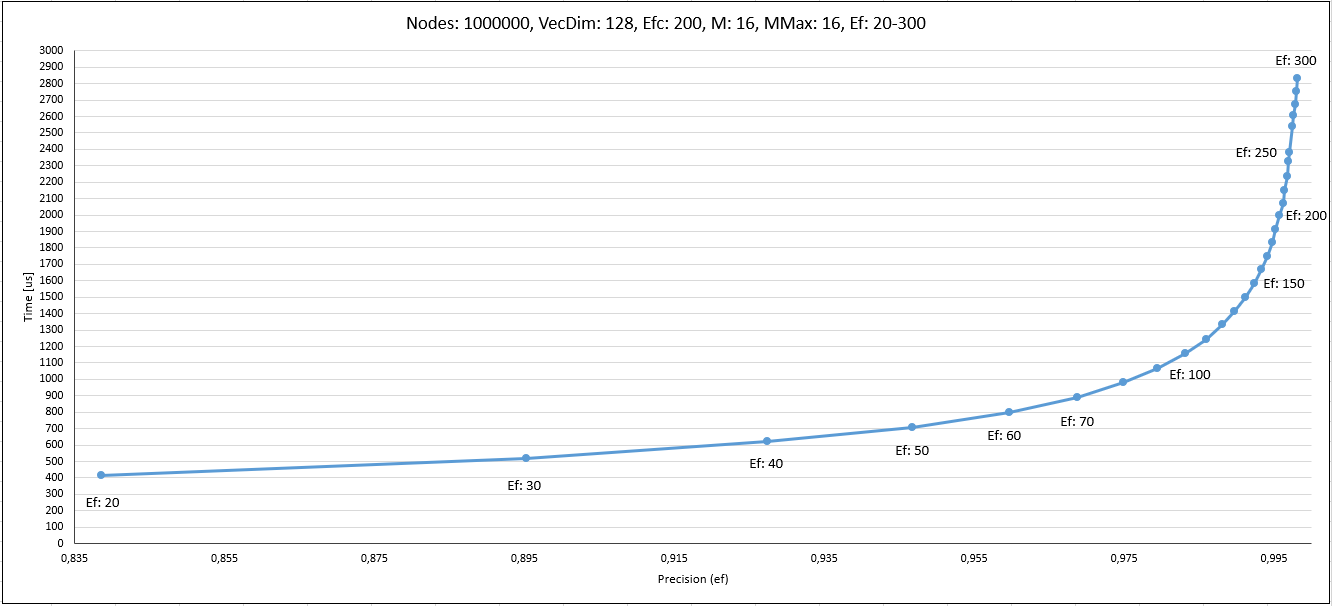
\includegraphics[scale=0.5]{Figures/graf_hnsw.png}
			\caption{Graf závislosti průměrného času jednoho dotazu na přesnosti}
			\label{graf_hnsw}
		\end{figure}
	
	\chapter{Filtr}
	\label{chap_filtr}
	
		Pod pojmem filtr si můžeme představit booleovskou podmínku omezující hodnoty jednotlivých atributů (dimenzí) prvků v n-dimenzionálním prostoru. Konkrétně tedy filtr říká jaké hodnotě se mají jednotlivé atributy rovnat, případně v jakém intervalu by se měly atributy pohybovat. Toto platí pouze pro atributy jež filtr omezuje, atributy které filtr nezmiňuje vůbec nekontrolujeme a akceptujeme je bez závislosti na jejich hodnotě.
		
		U KNN slouží filtr pro omezení vyhledání výsledných K prvků. Při vyhledávání výsledku se prochází i prvky které filtru nevyhovují, ale do vráceného výsledku jsou vloženy pouze prvky jejichž atributy vyhovují omezení filtru.
		
		Selektivita filtru \cite{OptINFORMIX} je číslo v rozsahu od 0 do 1 a udává procentuální počet prvků, které filtr přijme. Čím více je filtr vybíravý tím bližší hodnota k 0 mu bude přiřazena a tím více je filtr selektivnější. Naopak filtry přijímající většinu prvků budou mít přiřazeny číslo blíže k 1 a jejich selektivita bude tedy klesat, s tím že filtry přijímající úplně všechny prvky budou mít hodnotu selektivity rovno 1.
		
		\section{Implementace filtru a využití v HNSW}
		
		Filtr se implementoval jako vector objektů třídy VecDim. Tato třída reprezentuje jeden atribut a obsahuje ID dimenze, číslo od 0 do (vecDim - 1), vectory hodnot kterým má atribut (daná dimenze) nabývat nebo intervaly (tuple hodnoty od do) ve kterých se má atribut nacházet. Filtr je tedy nakonec vector který pro všechny atributy které chceme omezovat obsahuje hodnoty a intervaly kterým daný atribut musí vyhovovat, tedy minimálně jedné z těchto hodnot. Atributy které nijak neomezujeme ve vectoru atributů vůbec nejsou, porovnáváme jen ty atributy které nás ve filtru zajímají, ty ostatní přeskakujeme. Pro ověření zda daný prvek vyhovuje filtru jsem vytvořil pomocnou třídu VecDimHelper která pro daný prvek (vector hodnot) vrátí zda vyhovuje filtru nebo ne. Tato pomocná třída také generuje filtry dle určitých kritérií nebo umožňuje parsovat filtry z textové podoby a naopak.
		
		V HNSW se filtr využívá u metody KNNFilter. Této metodě oproti její verzi bez filtru musíme tedy krom $Q$, K a Ef předat i samotný filtr. Následně funguje stejně jen s tím rozdílem že používá vlastní SearchLayerFilter pro získání $F$ nejbližších prvků. Tato metoda funguje obdobně jako její verze bez filtru SearchLayerKNN. Rozdíl v implementaci s filtrem je v tom že nevracíme $W$ nejbližších nalezených prvků ale $F$ nejbližších nalezených prvků které zároveň vyhovují filtru. Na začátku tedy do $F$ uložíme entryPoint (jediný prvek v $W$) pokud splňuje podmínku filtru v opačném případě začíná průchod jako v popsaném Search v sekci HNSW (viz Kapitola \ref{MS}). Rozdíl je v tom že jedna z ukončovacích podmínek průchodu je původně vzdálenost nejbližšího prvku z $C$ je větší než vzdálenost nejvzdálenějšího prvku z $W$, v případě SearchLayerFilter je tato ukončovací podmínka rozšířena o to že zároveň musí platit že velikost $F$ je rovna zadanému K. Tím pádem je zaručeno že při průchodu se prvky prochází dokud nenalezneme K hledaných prvků vyhovujících filtru nebo již nemáme co procházet a $C$ je prázdné. Následně je ještě algoritmus rozšířen o část ve které do $F$ vkládáme nově nalezené prvky $e$ ($e$ jsou sousedi nejbližších prvků $c$ z $C$) pokud tento prvek filtr přijímá a zároveň je vzdálenost $e$ menší než vzdálenost nejvzdálenějšího prvku z $F$ nebo je velikost $F$ menší než K.
		
		\section{Měření HNSW implementace s filtrem}
		
		Při měření se provádělo 1000 testů pro každé K a různé selektivity, z výsledků těchto testů se následně získával průměr. U rozšířené KNNFilter implementace s filtrem (F) byla hodnota Ef nastavena pevně na 200. U implementace bez filtru (B) získáváme z metody KNN Kb prvků, a v těchto prvcích následně kontrolujeme zda se v nich nachází alespoň K prvků vyhovujících filtru a ty následně vracíme jako výsledek. Implementace bez filtru měla Ef nastavené také na 200, ale pokud v získaném Kb nebylo alespoň K prvků vyhovujících filtru, tak se zvedalo Kb, a pokud bylo $Kb > Ef$ tak se hodnota Ef nastavovala na hodnotu Kb (Ef nemůže být nikdy menší než K protože z nalezeného Ef se vrací K nejbližších prvků). Pro získání filtrů s určitou selektivitou se provádělo náhodné generování filtrů, spočítání kolika prvkům z celkových dat filtry vyhovují a pokud selektivity spadaly do požadovaných hranic tak se textové reprezentace filtrů ukládaly do souborů a následně se použili při testování. Veškeré výsledky testů jsou zaznamenány v tabulce (viz Tabulka \ref{FBC}).
		
		V tabulce (viz Tabulka \ref{FBC}) lze vidět že čím nižší je selektivita filtru tím kratší dobu operace KNN zabírá u implementace s filtrem i bez něj. Dokonce při $K << Ef$ dochází k tomu že filtry se selektivitou 50\%, 75\% a 90\% mají prakticky stejné časy u jednotlivých implementací. Je tomu tak protože ve vyhledaném Ef prvků se nalezne požadované K které vyhovuje filtru a tím pádem není potřeba provádět průchody navíc pro dohledání potřebného počtu prvků do K. Konkrétně pro $K = 10, Ef = 200$ trvá KNN přibližně 2,8ms pro všechny selektivity u implementace s filtrem (F). Implementace bez filtru (B) je obecně rychlejší při nízkém K a selektivitě od 50\% do 90\% za předpokladu že známe požadované potřebné Kb ve kterém najdeme K hledaných prvků, což by v praxi úplně neplatilo protože nevíme kolik přesně prvků musíme vrátit a muselo by tedy dojít k přibližným odhadům případně k opakovanému vyhledávání. Implementace B má čas operace přibližně 2,1ms pro nízké selektivity, 2,7ms pro selektivitu 25\% což je srovnatelné s časem 2,8ms u implementace F. Každopádně u vysokých selektivit vidíme že implementace F se vyplatí, má totiž 2,3x lepší čas než implementace B, konkrétně 3ms oproti 7ms. Stejně tak při stoupajícím K a konstantním Ef můžeme vidět že implementace F má lepší časy KNN operací než B i pro nižší selektivity.
		
		Z grafů porovnání průměrného času KNN operace implementace s a bez filtru pro různá K (viz Obrázek \ref{graf_filtr_all}) můžeme vidět již zmíněné chování. Tedy to že když známe Kb pro impl. B tak pro K = 10 (viz Obrázek \ref{graf_filtr_k10}) je impl. F rychlejší pouze pro vysokou selektivitu 10\%. S rostoucím K = 50 (viz Obrázek \ref{graf_filtr_k50}) je impl. F rychlejší až do selektivity  25\%. Při K = 100 (viz Obrázek \ref{graf_filtr_k100}) je impl. F rychlejší až do selektivity 50\% a nakonec u K = 200 (viz Obrázek \ref{graf_filtr_k200}) je impl. F rychlejší až do 75\% s tím že u selektivity 90\% mají impl. F i B relativně srovnatelné časy 3,05ms (F) a 2,81ms (B). Každopádně pro vysoké selektivity okolo 10\% je impl. F vždy rychlejší pro jakékoliv K než impl. B i když známe potřebné Kb pro impl. B.
		
		Dále lze vidět že s rostoucím K a konstantním Ef se stává že získaný počet KNN v implementaci F je o něco málo menší než bylo požadované K a je proto potřeba Ef postupně zvyšovat při rostoucím K (viz Kapitola \ref{FP}). Implementace s filtrem vrací obdobné výsledky jako ta bez filtru, pokud se získané výsledky liší tak kvůli tomu že implementace bez filtru vyhledává až příliš prvků (může mít mnohem vyšší Ef) a tím pádem zahodí ty prvky které jsou daleko od $Q$ a implementace s filtrem si tyto prvky ponechala a ukončila se jakmile našla požadované K v Ef prvcích.
		
		\newpage
		
		\begin{center}
			
			\begin{tabular}{c c c c c c c c}\label{FBC}
				
				Sel[\%] & tF[us] & tB[us] & Shoda FB & Získ. KNN u F & Prům. potř. Kb u B \\
				\midrule
				K: 10\\
				10 & 3040,97 & 7056,26 & 0,91 & 10,00 & 715,28\\
				25 & 2867,57 & 2703,60 & 0,99 & 10,00 & 124,00\\
				50 & 2817,17 & 2168,04 & 1,00 & 10,00 & 25,96\\
				75 & 2805,95 & 2163,28 & 1,00 & 10,00 & 15,83\\
				90 & 2811,61 & 2163,50 & 1,00 & 10,00 & 13,34\\
				K: 50\\
				10 & 3534,66 & 16451,46 & 0,73 & 49,67 & 1800,22\\
				25 & 3076,86 & 4966,35 & 0,93 & 49,96 & 426,49\\
				50 & 2921,99 & 2435,99 & 0,99 & 50,00 & 105,44\\
				75 & 2903,95 & 2129,43 & 1,00 & 50,00 & 71,57\\
				90 & 2891,03 & 2113,17 & 1,00 & 50,00 & 58,76\\
				K: 100\\
				10 & 3961,65 & 25212,24 & 0,58 & 98,77 & 2747,15\\
				25 & 3268,71 & 8161,75 & 0,85 & 99,88 & 753,35\\
				50 & 2999,55 & 2952,85 & 0,97 & 100,00 & 221,45\\
				75 & 2946,42 & 2226,74 & 1,00 & 100,00 & 160,95\\
				90 & 2930,98 & 2117,40 & 1,00 & 100,00 & 142,65\\
				K: 150\\
				10 & 4292,07 & 32129,19 & 0,50 & 147,38 & 3547,55\\
				25 & 3411,34 & 11481,21 & 0,76 & 149,78 & 1060,20\\
				50 & 3089,03 & 3804,70 & 0,95 & 150,00 & 319,30\\
				75 & 3036,32 & 2642,55 & 0,98 & 150,00 & 226,25\\
				90 & 2992,38 & 2173,99 & 1,00 & 150,00 & 197,20\\
				K: 200\\
				10 & 4578,50 & 37901,86 & 0,45 & 195,29 & 4234,40\\
				25 & 3587,91 & 14764,61 & 0,68 & 199,68 & 1367,60\\
				50 & 3175,45 & 5156,43 & 0,90 & 200,00 & 417,50\\
				75 & 3096,15 & 3594,97 & 0,95 & 200,00 & 290,35\\
				90 & 3051,25 & 2810,96 & 0,99 & 200,00 & 251,65\\
				\\
			\end{tabular}
			
			{\footnotesize *F = impl. KNN s filtrem, B = impl. KNN bez filtru, sel = selektivita filtru, tF = prům. čas F, tB = průměrný čas B, Shoda FB = shoda získaných prvků z F a B, Získ. KNN u F = prům. počet získaných prvků ze zvoleného K u F, Prům. potř. Kb u B = průměrný počet zadaného Kb v B pro získání K prvků}\\
			
			\captionof{table}{Porovnání vlastností u implementase KNN s filtrem a bez filtru}
			
		\end{center}
		
		\label{graf_filtr_all}
		\begin{figure}
			\centering
			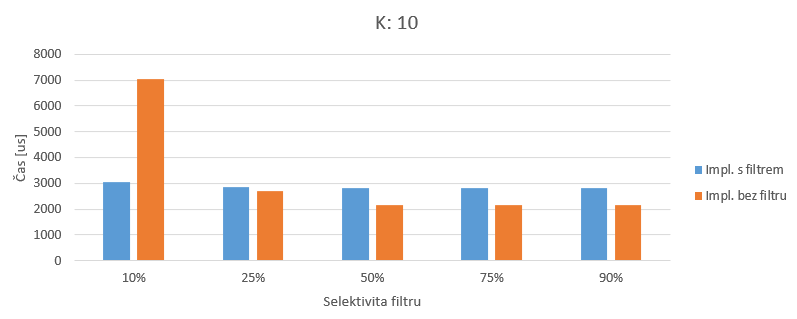
\includegraphics[scale=0.8]{Figures/graf_filtr_k10.png}
			\caption{Porovnání průměrného času operace u implementací F a B, K: 10}
			\label{graf_filtr_k10}
		\end{figure}
	
		\begin{figure}
			\centering
			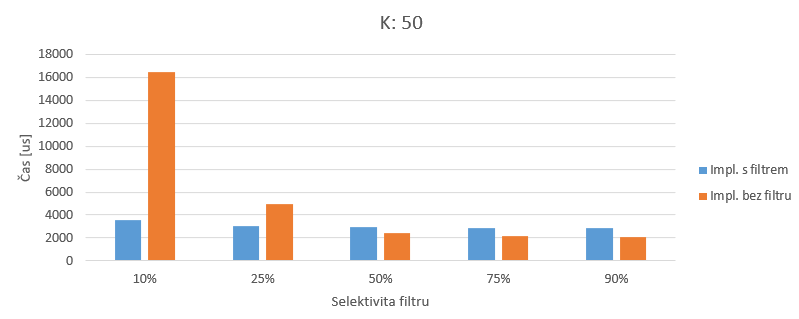
\includegraphics[scale=0.8]{Figures/graf_filtr_k50.png}
			\caption{Porovnání průměrného času operace u implementací F a B, K: 50}
			\label{graf_filtr_k50}
		\end{figure}
	
		\begin{figure}
			\centering
			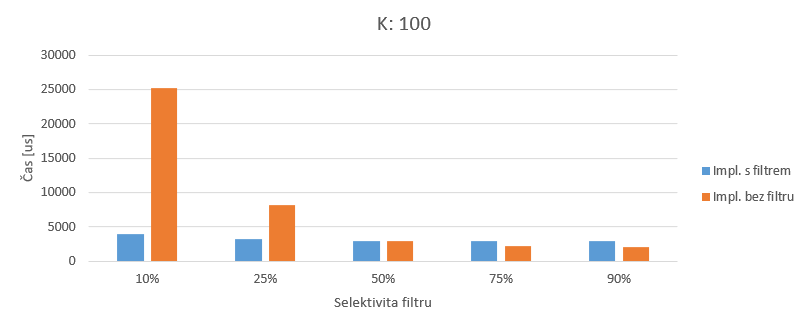
\includegraphics[scale=0.8]{Figures/graf_filtr_k100.png}
			\caption{Porovnání průměrného času operace u implementací F a B, K: 100}
			\label{graf_filtr_k100}
		\end{figure}
	
		\begin{figure}
			\centering
			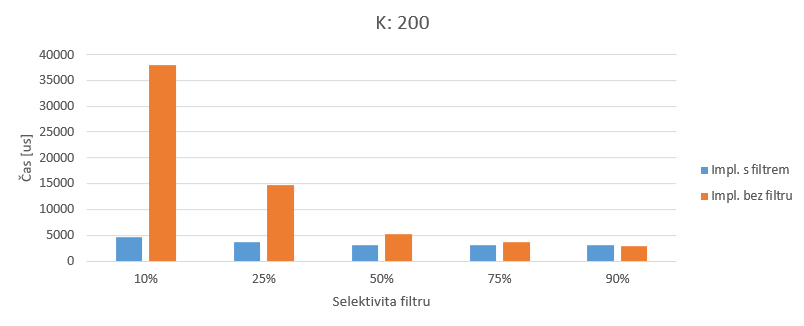
\includegraphics[scale=0.8]{Figures/graf_filtr_k200.png}
			\caption{Porovnání průměrného času operace u implementací F a B, K: 200}
			\label{graf_filtr_k200}
		\end{figure}
		
		\section{Problém filtru s vysokou selektivitou u HNSW}
		\label{FP}
		
			Při použití implementace HNSW s využitím filtru se může stát že nám metoda KNNFilter nevrátí K hledaných prvků, ale výsledný počet hledaných prvků bude o něco málo nižší (viz Tabulka \ref{FBC}). Pokud tomu nastane tak nám ve výsledku chybí nízký počet prvků, nejčastěji 1 nebo 2 ale pravděpodobnost že k tomuto jevu dojde je relativně nízká.
			
			Tento jev nastává ve chvíli kdy hodnota K je stejně vysoká nebo jen o něco málo nižší než Ef a zároveň je selektivita filtru vyšší, do 25\%.
			
			K tomuto problému dochází protože HNSW algoritmus pro procházení grafu a nalezení nejbližších prvků použitý v metodě SearchKNNFilter lze zakončit dvěma způsoby. První způsob jak zakončit algoritmus průchodu který nás aktuálně nezajímá je ten kdy vzdálenost nejbližšího prvku z $C$ je vyšší než vzdálenost nejvzdálenějšího prvku z $W$ a zároveň je počet prvků v $F$ (původně $W$) roven zadanému K.
			
			Druhý způsob jak ukončit průchod, ten který způsobí problém, je ten kdy je $C$ prázdný. Stane se tedy že projdeme prvky z $C$ a všechny jejich nenavštívené sousedy kteří jsou blíže než nejvzdálenější prvek z $W$. Během tohoto průchodu jednoduše nenarazíme na dostatečný počet prvků které by vyhovovaly filtru a $F$ obsahuje tedy méně nejbližších prvků než je počet co hledáme.
			
			Tento problém lze jednoduše vyřešit tím že zvýšíme hodnotu Ef aby byla více rozdílná a vyšší než hodnota K. S rostoucím Ef při zachování K a filtru poroste i čas vykonání operace, ale bude se i zvyšovat pravděpodobnost že získáme přesně K hledaných prvků.
	
	\chapter{Závěr}
	\label{chap_zaver}
	
		K závěru bych řekl že část práce určená pochopení a implementaci HNSW byla mnohem pracnější než následné rozšíření o filtry. Je tomu tak protože jsem pro lepší pochopení HNSW celý projekt psal od začátku a následné rozšíření nevyžaduje mnoho nových implementací. Stačí prakticky jen již naimplementované algoritmy rozšířit o pár podmínek. Každopádně volba naimplementovat si projekt znovu sám byla určitě správná, protože i přes různé komplikace mi toto rozhodnutí dovolilo skvěle pochopit myšlenky a principy HNSW.
		
		Dále bych chtěl zmínil že implementace takovýchto problémů má velice složité debugování a to hned z několika důvodů. Data jsou obrovská a stává se že implementace je obdobná s referencí do doby než se vloží prvek který je v datech daleko. Zabírá to hlavně spoustu času z důvodu dlouhého vytváření grafů a následného hledání kde přesně konkrétně došlo k rozdílu. Ve finální implementaci se využívá i náhodné vybrání vrstev a dokonce pokud dva prvky mají stejnou vzdálenost tak může dojít k rozdílným výsledkům. Problém je zapříčiněn i tím že data jsou reprezentována pomocí grafů s mnoha sousedy, což znamená že kód s podstatnou chybou působí dlouho jako správný a k rozdílu dojde až při vložení velkého množství prvků, nebo správného prvku který chybu způsobí.
		
		V práci jsem až moc častou využíval std::vector, použití jednoduchých polí ať už staticky nebo dynamicky alokovaných by přineslo v určitých místech lepší propustnosti při správném využití nebo by graf zabíral méně paměti.
		
		Práce mi určitě přinesla lepší pochopení C++, manipulaci s daty a důležitost jednotlivých rozhodnutí ohledně využití datových struktur nebo algoritmů pro zlepšení výsledné propustnosti a potřebné paměti. Projekt mě bavil a mimo složitý debug jsem si i práci užil. Jsem tedy spokojený že si tento projekt zvolil. KNN je důležitý problém a HNSW je zajímavý, jednoduchý a zároveň efektivní způsob jak jej za určitých podmínek efektivně řešit.
	
	\nocite{*}
	
	\printbibliography[title={Literatura}, heading=bibintoc]
	
\end{document}]